%%%%%%%%%%%%%%%%%%%%%%%%%%%%%%%%%%%%%%%%%%%%%%%%%%%%%%%%%%%%
% Document settings
\documentclass{ACGSeminar}

\bibliography{references}

%%%%%%%%%%%%%%%%%%%%%%%%%%%%%
% Hyphenations here
%%%%%%%%%%%%%%%%%%%%%%%%%%%%%
\hyphenation{}

%%%%%%%%%%%%%%%%%%%%%%%%%%%%%
% Title, Author, etc.

\begin{document}

\title{Efficient Ray Tracing Techniques}

\author{Dario Seyb}

\maketitle

%%%%%%%%%%%%%%%%%%%%%%%%%%%%%%%%%%%%%%%%%%%%%%%%%%%%%%%%%%%%
% Abstract

\begin{abstract}%
Ray Tracing is next to rasterization the most widely used technique to generate discrete 2D images from continuous 3D scenes. Until recently ray tracing was too resource intensive to produce images in realtime, but advances in hardware capabilities, most notably the introduction of GPGPU (General Purpose Graphics Processing Units), and algorithms made near-realtime ray tracing feasible. In this report we will present some of the techniques which are used to achieve this.
\end{abstract}

\keywords{Ray Tracing, Acceleration Structures, Realtime Rendering, GPGPU}
\tableofcontents

%%%%%%%%%%%%%%%%%%%%%%%%%%%%%%%%%%%%%%%%%%%%%%%%%%%%%%%%%%%%
% Introduction

\section{Introduction}

Introduction to your exciting topic including
some citation~\cite{Pharr:2010:PBR:1854996}. Define citations
in \verb+references.bib+ that you find in
the latex source folder.

%%%%%%%%%%%%%%%%%%%%%%%%%%%%%%%%%%%%%%%%%%%%%%%%%%%%%%%%%%%%
% Second Section

\section{A brief history of ray tracing}
Talk about ray tracing from Whitted to Hyperion.

\section{Overview over the path tracing algorithm}
A short overview of the base algorithm we are going to use for the rest of the paper. Cite \cite{veach1997robust} all the way.

\section{Spacial partitioning and acceleration structures}
Going logarithmic baby!
\subsection{BSP and KD-Trees}
\subsection{Volume Hierachies}

\section{Accelerating the convergence of path tracing}
Here's where \cite{Pharr:2010:PBR:1854996} comes in.
\subsection{Bidirectional Path Tracing}
\subsection{Gradient-Domain Path Tracing}
Do I really wanna go here? \cite{Kettunen2015sg}

\section{Adapting the described algorithms to the GPU}
\subsection{Accessing the GPU outside of the rasterization pipeline}
\subsection{Hierarchical data structures on the GPU}

\section{Results}
\subsection{Images}
\subsection{Timings}

\begin{figure}[htb!]
  \begin{centering}
    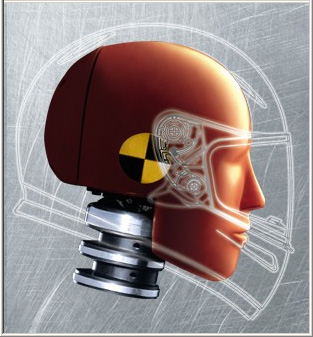
\includegraphics[width=4cm]{figures/dummy.jpg}\par
  \end{centering}
  \caption{A simple dummy picture to demonstrate how
           to include graphics into your report.}
  \label{fig:dummy}
\end{figure}

%%%%%%%%%%%%%%%%%%%%%%%%%%%%%%%%%%%%%%%%%%%%%%%%%%%%%%%%%%%%
% Bibliography

\printbibliography
\cleardoublepage

\end{document}
